\documentclass{article}
\usepackage{spconf,amsmath,amssymb,graphicx,booktabs,array,microtype,dblfloatfix,float}
\graphicspath{{figures_icassp/}{figures_nested/}}
% Automatically generated from outputs/icassp_primary/summary.csv.
\newcommand{\PixelFisherRange}{0.277--0.520}
\newcommand{\CaseSpearmanRange}{0.890--0.966}
\newcommand{\NAURCRange}{0.024--0.092}
\newcommand{\RRRFiftyRange}{19.3--52.1\%}

% Automatically generated from outputs/shared_error_stress/summary.csv.
\newcommand{\StressMaeIncrease}{14.9\%}
\newcommand{\StressTargetIncrease}{28.6\%}
\newcommand{\StressSharedChange}{0.0\%}
\newcommand{\StressCommitteeMaeIncrease}{11.8\%}

\newcommand{\NestedInteractionCount}{561,492}
\newcommand{\NestedRetainedCount}{1,320}
\newcommand{\NestedBaselineNAURC}{0.077}
\newcommand{\NestedTriageNAURC}{0.052}
\newcommand{\NestedLowNAURC}{0.050}
\newcommand{\NestedBaselineRho}{0.884}
\newcommand{\NestedTriageRho}{0.911}
\newcommand{\NestedLowRho}{0.908}
\newcommand{\NestedBaselineRRR}{21.9\%}
\newcommand{\NestedTriageRRR}{21.4\%}
\newcommand{\NestedLowRRR}{21.6\%}
\newcommand{\NestedDeltaNAURC}{-0.026}
\newcommand{\NestedDeltaNAURCLo}{-0.063}
\newcommand{\NestedDeltaNAURCHi}{-0.001}
\newcommand{\NestedAttrAdv}{0.060}
\newcommand{\NestedAttrWithin}{0.126}
\newcommand{\NestedAttrTop}{27.3\%}
\newcommand{\NestedMeanNeural}{0.08}
\newcommand{\NestedLowMeanNeural}{0.04}
\newcommand{\PhysicalMatchedRecords}{1,518}

\setlength{\textfloatsep}{6pt plus 2pt minus 2pt}
\setlength{\dbltextfloatsep}{6pt plus 2pt minus 2pt}
\setlength{\floatsep}{5pt plus 2pt minus 2pt}
\setlength{\intextsep}{5pt plus 2pt minus 2pt}
\setlength{\tabcolsep}{2.7pt}
\renewcommand{\arraystretch}{0.94}
\makeatletter
\let\oldthebibliography\thebibliography
\renewcommand{\thebibliography}[1]{\oldthebibliography{#1}\setlength{\itemsep}{11.8pt plus 0.6pt minus 0.5pt}\setlength{\parsep}{0pt}\setlength{\parskip}{0pt}}
\makeatother

\title{MULTISCALE RELIABILITY RANKING OF MRI SLICE INTERPOLATION:\\
EXTENDED ANALYSIS OF COMMITTEES, ATTRIBUTION, AND PHYSICAL CONSISTENCY}
\name{Anonymous Authors}
\address{Anonymous submission}

\begin{document}
\ninept
\maketitle

\begin{abstract}
Cohort-average fidelity cannot identify which MRI slice interpolation should be reviewed when the missing target is unavailable. We study two ground-truth-free ranking signals from deterministic outputs: target-to-committee disagreement, which excludes the target reconstructor, and same-target consistency on physical planes generated at multiple interpolation factors. Ground truth defines only retrospective error labels. Experiments include 115 IXI, 24 fastMRI-brain, and 22 eight-fold out-of-fold NingXia T2 examinations; the latter two are evaluated at $\times2/\times4/\times6$. On nine fixed NingXia factor--target profiles, physical consistency changes mean nAURC from \NestedBaselineNAURC\ to \NestedTriageNAURC\ and Spearman correlation from \NestedBaselineRho\ to \NestedTriageRho; the profile-aligned paired nAURC difference is \NestedDeltaNAURC\ [\NestedDeltaNAURCLo, \NestedDeltaNAURCHi]. Conversely, nested target/scale-specific selection over \NestedInteractionCount\ registered score--committee interactions does not outperform the frozen baseline, and calibrated target attribution remains weak. Shared errors cancel from cross-model disagreement. These scores rank selective review; neither is a calibrated probability or clinical guarantee.
\end{abstract}

\begin{keywords}
MRI interpolation, reliability ranking, selective review, model disagreement, multiscale consistency
\end{keywords}

\section{Introduction}
Through-plane interpolation densifies sparse MRI stacks for visualization, registration, and volumetric processing. Modern methods model inter-slice context or adapt restoration transformers \cite{song2024i3net,liang2021swinir,chen2022hat}, yet are usually compared by cohort-average PSNR, SSIM, or MAE. Such summaries cannot identify an unreliable examination after the missing target slice becomes unobservable.

Model-internal uncertainty uses stochastic inference, repeated training, heteroscedastic objectives, test-time augmentation (TTA), or learned error prediction \cite{gal2016dropout,lakshminarayanan2017deepensembles,kendall2017uncertainties,wang2018tta,edupuganti2021uqmri,hu2021predict,zhang2024trainingfree}; no-reference MRI quality assessment instead targets perceptual quality or acquisition artifacts \cite{stepien2022nriqa}. Our operational setting assumes only deterministic interpolator outputs and asks whether they rank examinations for selective review \cite{elyaniv2010selective,geifman2019selectivenet,ding2020aurc}. Heterogeneous outputs provide cross-model evidence, while reconstructions of the same source stack at known factors provide a second signal when their generated planes coincide physically.

We contribute: (1) a target-excluded reliability-ranking protocol augmented by physical-plane cross-scale consistency; (2) a leakage-controlled evaluation with common-support fidelity, \NestedInteractionCount\ registered score--committee interactions, eight-fold nested selection, calibrated target attribution, and profile-aligned bootstrap; and (3) empirical boundaries showing that fixed disagreement transfers better than high-flexibility adaptive selection, while shared errors remain invisible. We claim error association and review ranking, not posterior uncertainty, diagnostic correctness, or clinical safety.

\section{Method}
\subsection{Target-to-committee disagreement}
Let $x$ be observed sparse-slice context, $y$ the unobserved dense target, and $\hat y_m=f_m(x)$ the output of target interpolator $m$. For available identities $\mathcal B$, define $\mathcal C_m=\{b\in\mathcal B:b\neq m\}$. All outputs must share case identity, source-intensity representation, affine, orientation, voxel grid, and generated-slice convention. At generated voxel $i$, the frozen map is
\begin{equation}
 U_m(i)=\mathop{\mathrm{median}}_{b\in\mathcal C_m}|\hat y_m(i)-\hat y_b(i)|.
 \label{eq:target}
\end{equation}
This is median target-to-member disagreement, not statistical median absolute deviation or posterior variance. Let $\mathcal G_r$ be slices generated at factor $r$. The deployment mask and examination score are
\begin{align}
 M_m(i)&=\mathbf1[|\hat y_m(i)|>0.01\max_{j\in\mathcal G_r}|\hat y_m(j)|],\nonumber\\
 s_m&=\frac{\sum_{i\in\mathcal G_r}M_m(i)U_m(i)}{\sum_{i\in\mathcal G_r}M_m(i)}. \label{eq:case}
\end{align}
Ground truth is inaccessible to Eqs.~\eqref{eq:target}--\eqref{eq:case}. Bank-union and observed-input masks, upper-tail pooling, gradient/Laplacian domains, relative differences, member weighting, trimming, and subset committees are registered alternatives.

\begin{figure}[!t]
 \centering
 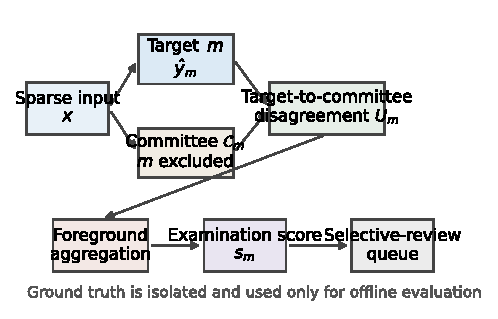
\includegraphics[width=0.98\columnwidth]{figure_framework_outlined.pdf}
 \caption{Ground-truth-free scoring and offline evaluation. The named target is excluded from its committee; missing targets are revealed only to the evaluator.}
 \label{fig:framework}
\end{figure}

\subsection{Physical cross-scale consistency}
Array depth alone does not determine whether factors can be compared. For NIfTI affine $A$, slice $z$ has world-plane origin $p(z)=A_{1:3,4}+A_{1:3,3}z$. For factors $r\neq r'$, we retain only planes generated in both reconstructions whose origins agree within $10^{-3}$ mm; no resampling is introduced. The same-target physical signal is
\begin{equation}
 C_m(p)=\mathop{\mathrm{median}}_{r\neq r'}|\hat y_m^{(r)}(p)-\hat y_m^{(r')}(p)|,
 \label{eq:physical}
\end{equation}
aggregated over a union foreground. We evaluate Eq.~\eqref{eq:physical} alone and the pre-defined rank hybrid $h_m=\tfrac12\operatorname{rank}(s_m)+\tfrac12\operatorname{rank}(C_m)$. Physical consistency requires reconstructions at multiple known factors, so it is most natural for cached retrospective audits; it is not a cheaper substitute for a single online reconstruction.

\subsection{Failure boundary and selective review}
Write $\hat y_b=y+c+\epsilon_b$, where $c$ is shared error and $\epsilon_b$ member-specific. Then $\hat y_m-\hat y_b=\epsilon_m-\epsilon_b$: disagreement responds to model-specific separation but exactly cancels any identical perturbation applied to all outputs. Consensus therefore cannot certify correctness.

For offline error $E_j$, examinations are retained by increasing score. At coverage $q$, $R(q)$ is retained mean MAE and $\mathrm{RRR}(q)=[R_{\rm random}-R(q)]/R_{\rm random}$. We report Spearman $\rho$ and $\mathrm{nAURC}=(\mathrm{AURC}-\mathrm{AURC}_{\rm oracle})/(\mathrm{AURC}_{\rm random}-\mathrm{AURC}_{\rm oracle})$, where zero is oracle and one expected random review. Coverage always means retained fraction.

\section{Experiments}
\subsection{Data, models, and governance}
The factor-four study uses IXI (115 examinations) \cite{ixi}, fastMRI-brain (24) \cite{zbontar2018fastmri}, and an internal NingXia T2 cohort (22) pooled from eight out-of-fold prediction folds. fastMRI-brain and NingXia also use the same identities at $\times2$ and $\times6$. Eleven neural reconstructors are audited: I$^3$Net, HAT, SwinIR, SAINT, SMamba-UNet, Pix2PixGAN, ResUNet, ResSRDiff, ArSSR, CycleINR, and ACVTT; linear and cubic interpolation are analytical references \cite{keys1981cubic,thevenaz2000interpolation}. All listed outputs pass case, shape, affine, finite-value, and generated-index checks.

Cross-model fidelity is recomputed on one offline ground-truth 1\% foreground and generated slices, rather than each model's own mask. Development-only composite ranks over MAE, MSE, PSNR, global SSIM, and NCC define six main targets and an architecture-constrained common bank of six neural plus two analytical members. No NingXia outer result changes these identities.

Broad screening uses IXI $\times4$ and fastMRI-brain $\times2/\times4/\times6$. We enumerate \NestedInteractionCount\ interactions over 18 intensity, structural, and pooling features, committee sizes 2--5/full, and six uniform, fidelity, diversity, combined, or trimmed weighting rules; stratified pruning retains \NestedRetainedCount. For each NingXia outer fold, the other seven folds select a target- and factor-conditioned candidate; the outer score is calibrated by its inner empirical CDF. A declared cost rank and one-standard-error simplicity rule are implemented. The first unconstrained pass and a prospectively recorded neural-peer amendment are both retained after neither transfers. Attribution calibration and relative centering are selected by matched advantage, within-case model ranking, and top-1 identification, not triage nAURC.

Every final profile contains all 22 outer predictions. We use 2,000 paired case-bootstrap replicates with fixed indices. Aggregate differences are computed within each replicate for every fixed factor--target profile and only then averaged across profiles. Thus profile bootstrap samples are never flattened. Failure-decile AUROC/AUPRC remain secondary.

\section{Results}
\begin{table}[!t]
 \centering
 \caption{NingXia outer-fold ranking, averaged over I$^3$Net, HAT, and SwinIR. Coverage is retained fraction; lower nAURC is better.}
 \resizebox{\columnwidth}{!}{\begin{tabular}{llccc}
\toprule
Factor & Method & $\rho$ [95\% CI] & nAURC [95\% CI] & RRR50 \\
\midrule
$\times$2 & Frozen baseline & 0.879 [0.749, 0.941] & 0.070 [0.033, 0.139] & 22.3\% \\
$\times$2 & Physical consistency & 0.878 [0.744, 0.946] & 0.075 [0.035, 0.150] & 20.6\% \\
$\times$2 & Fixed rank hybrid & 0.886 [0.757, 0.949] & 0.066 [0.030, 0.133] & 20.6\% \\
$\times$2 & Mean disagreement & 0.893 [0.770, 0.953] & 0.064 [0.028, 0.130] & 22.0\% \\
$\times$4 & Frozen baseline & 0.912 [0.820, 0.945] & 0.063 [0.031, 0.142] & 22.2\% \\
$\times$4 & Physical consistency & 0.934 [0.852, 0.964] & 0.053 [0.026, 0.096] & 21.6\% \\
$\times$4 & Fixed rank hybrid & 0.934 [0.855, 0.965] & 0.034 [0.019, 0.093] & 22.2\% \\
$\times$4 & Mean disagreement & 0.915 [0.819, 0.949] & 0.057 [0.028, 0.129] & 22.2\% \\
$\times$6 & Frozen baseline & 0.862 [0.730, 0.920] & 0.098 [0.049, 0.184] & 21.2\% \\
$\times$6 & Physical consistency & 0.922 [0.814, 0.972] & 0.026 [0.010, 0.058] & 22.0\% \\
$\times$6 & Fixed rank hybrid & 0.906 [0.792, 0.950] & 0.051 [0.024, 0.097] & 22.1\% \\
$\times$6 & Mean disagreement & 0.843 [0.704, 0.903] & 0.122 [0.062, 0.219] & 20.2\% \\
\bottomrule
\end{tabular}
}
 \label{tab:nested}
\end{table}

\begin{figure*}[!t]
 \centering
 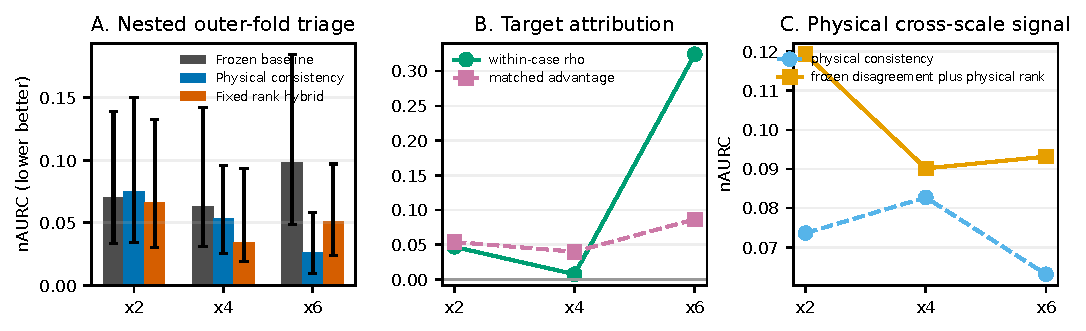
\includegraphics[width=0.98\textwidth]{nested_multiscale_results.pdf}
 \caption{Outer-fold evidence. (A) Fixed cross-model baseline, physical consistency, and their rank hybrid. (B) Attribution after inner-fold target calibration. (C) Physical consistency and hybrid across all audited targets. Error bars in (A) are profile-aligned 95\% bootstrap intervals.}
 \label{fig:nested}
\end{figure*}

\subsection{Physical consistency improves examination ranking}
All \PhysicalMatchedRecords\ audited case--target--scale-pair records contain at least one common generated physical plane. On the nine primary NingXia profiles, Eq.~\eqref{eq:physical} improves mean nAURC from \NestedBaselineNAURC\ to \NestedTriageNAURC\ and $\rho$ from \NestedBaselineRho\ to \NestedTriageRho\ (Table~\ref{tab:nested}, Fig.~\ref{fig:nested}). The profile-aligned paired nAURC change is \NestedDeltaNAURC\ [\NestedDeltaNAURCLo, \NestedDeltaNAURCHi]. The fixed hybrid has nAURC \NestedLowNAURC\ and RRR50 \NestedLowRRR; its difference from consistency alone is inconclusive. This supports complementary physical evidence, not probability calibration.

\subsection{Adaptive selection and attribution do not transfer}
The frozen baseline obtains nAURC \NestedBaselineNAURC, $\rho=\NestedBaselineRho$, and RRR50 \NestedBaselineRRR. Mean disagreement is nearly identical, so the median aggregator is not claimed as a unique algorithmic advance. In contrast, the unconstrained nested selector collapses mostly to Linear+Cubic under one-SE and obtains nAURC 0.282; requiring neural peers and adding public-development stability yields 0.323. Both failures remain registered. The result argues for a simple frozen default when labeled inner folds are tiny, rather than dataset-specific committee claims.

Target-calibrated attribution has mean matched advantage \NestedAttrAdv, within-case $\rho=\NestedAttrWithin$, and top-1 accuracy \NestedAttrTop. It is stronger at $\times6$ but weak overall; examination difficulty, rather than target identity, explains most score variation. We therefore present target attribution as a boundary, not a validated deployment claim.

\subsection{Shared errors, cost, and scope}
In the controlled IXI stress test, maximum-strength target-only corruption raises disagreement by \StressTargetIncrease, whereas applying the identical corruption to all outputs changes disagreement by only \StressSharedChange\ despite increasing reconstruction error (Fig.~\ref{fig:stress}). This verifies common-mode invariance, not clinical realism.

\begin{figure}[H]
 \centering
 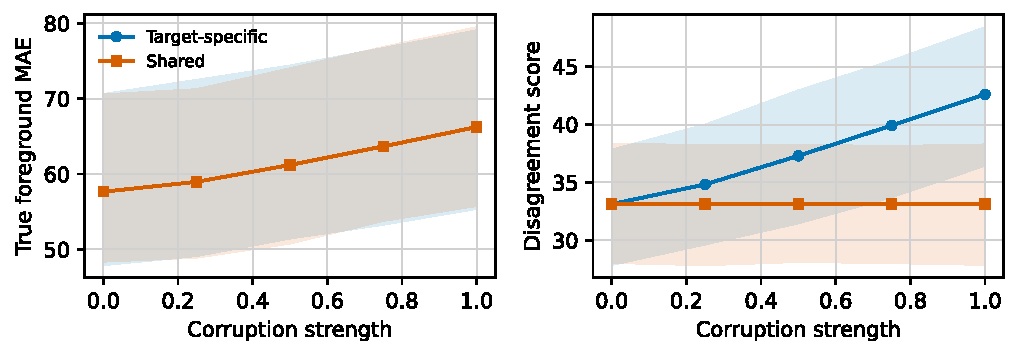
\includegraphics[width=0.96\columnwidth]{shared_error_stress_outlined.pdf}
 \caption{Target-specific corruption raises error and disagreement; identical shared corruption raises error while cancelling from cross-model differences. Bands are 95\% bootstrap intervals.}
 \label{fig:stress}
\end{figure}

Stored-output cross-model scoring takes 1.18 s mean per examination on CPU with 0.89 GiB peak RSS. Physical consistency adds comparisons but, online, requires two additional factor-specific executions of the target model; the hybrid also requires committee outputs. Thus cross-model scoring suits cached audits, while physical consistency trades more reconstruction cost for improved multiscale ranking.

\clearpage
\section{Extended Model-Bank and Fidelity Audit}
The original fidelity screen compared each model on its own prediction-derived foreground. That support changes with the model and can reward a reconstructor that suppresses difficult tissue. We therefore recompute every metric on the same generated-slice ground-truth foreground for development selection only. This ground-truth support is inaccessible to deployment scoring and never defines the reported reliability score.

\begin{table*}[!t]
 \centering
 \caption{Corrected fastMRI-brain development fidelity, averaged equally over $\times2/\times4/\times6$. Rank is the pre-defined composite of common-support MAE, MSE, PSNR, global SSIM, and NCC; ``old'' used model-specific masks.}
 \resizebox{0.82\textwidth}{!}{\begin{tabular}{r l r r r r r}
\toprule
Rank & Model & MAE & PSNR & SSIM & NCC & Old rank \\
\midrule
1 & i3net & 66.03 & 19.80 & 0.881 & 0.885 & 1 \\
2 & saint & 81.03 & 18.32 & 0.847 & 0.850 & 2 \\
3 & hat & 83.62 & 18.07 & 0.830 & 0.836 & 6 \\
4 & smamba\_unet & 83.92 & 18.02 & 0.827 & 0.834 & 3 \\
5 & pix2pixgan & 81.55 & 18.16 & 0.840 & 0.840 & 4 \\
6 & swinir & 84.60 & 17.99 & 0.823 & 0.831 & 5 \\
7 & resunet & 86.11 & 17.84 & 0.825 & 0.830 & 7 \\
8 & ressrdiff & 95.80 & 16.82 & 0.788 & 0.793 & 8 \\
9 & arssr & 107.42 & 16.02 & 0.694 & 0.715 & 10 \\
10 & cycleinr & 107.63 & 16.00 & 0.693 & 0.714 & 9 \\
11 & acvtt & 114.86 & 15.77 & 0.691 & 0.709 & 11 \\
12 & linear & 127.29 & 14.81 & 0.621 & 0.629 & -- \\
13 & cubic & 138.81 & 14.09 & 0.597 & 0.597 & -- \\
\bottomrule
\end{tabular}
}
 \label{tab:fidelity-full}
\end{table*}

Table~\ref{tab:fidelity-full} changes HAT from rank 6 to 3, SMamba-UNet from 3 to 4, Pix2PixGAN from 4 to 5, SwinIR from 5 to 6, and exchanges ArSSR/CycleINR at ranks 9--10. The six main targets are I$^3$Net, SAINT, HAT, SMamba-UNet, Pix2PixGAN, and SwinIR. The common-bank candidate pool uses these six neural methods plus Linear and Cubic; the named target is removed at scoring. This is an availability-conditioned common-bank rule, not a fixed universal committee.

The best reconstructor need not be the best peer. Analytical methods rank lowest in fidelity but can expose low-frequency or oversmoothing departures at negligible CPU cost. Conversely, two high-fidelity transformers may be redundant. The search therefore treats fidelity, output diversity, architecture family, and cost as separate quantities rather than assuming a monotonic relation.

\section{Extended Candidate Search}
The 18 retained atomic features comprise intensity mean, 90th percentile, top-10\% mean, maximum-slice, slice-90th-percentile, and top-two-slice pooling under bank-union support; intensity mean/90th/top-10\% under target-1\% and input-derived supports; relative mean/90th; gradient mean/90th; Laplacian mean; and local-energy-normalized mean. For the architecture-constrained bank we enumerate committee sizes 2, 3, 4, 5, and full. Uniform, inverse-fidelity, exponential fidelity-rank, error-complement diversity, combined fidelity/diversity, and remove-most-distant aggregation yield \NestedInteractionCount\ registered interactions.

Weighted interaction candidates aggregate target--member case features and are interpreted as robust weighted disagreement, whereas the frozen baseline recomputes the voxelwise committee median in Eq.~\eqref{eq:target}. This distinction is retained in the registry. Stratified pruning keeps the five best and three simplest candidates per target, factor, and score family, yielding \NestedRetainedCount\ nested candidates rather than a global top-$k$ funnel.

\begin{table}[!t]
 \centering
 \caption{Unconstrained first-pass nested choices. Neural is the mean number of neural peers selected across outer folds and all audited targets.}
 \resizebox{\columnwidth}{!}{\begin{tabular}{llccll}
\toprule
Role & Factor & Neural & Total & Modal score & Weight \\
\midrule
Nested triage & $\times$2 & 0.06 & 2.00 & intensity\_slice\_max\_\_bank\_union & uniform \\
Nested triage & $\times$4 & 0.08 & 2.03 & gradient\_q90\_\_bank\_union & uniform \\
Nested triage & $\times$6 & 0.09 & 2.02 & intensity\_mean\_\_bank\_union & uniform \\
Nested low-cost & $\times$2 & 0.06 & 2.00 & intensity\_slice\_max\_\_bank\_union & uniform \\
Nested low-cost & $\times$4 & 0.05 & 2.01 & gradient\_q90\_\_bank\_union & uniform \\
Nested low-cost & $\times$6 & 0.02 & 2.00 & intensity\_mean\_\_bank\_union & uniform \\
\bottomrule
\end{tabular}
}
 \label{tab:selection-full}
\end{table}

For candidate $c$, the declared first-pass objective is
\begin{equation}
 J(c)=R_{\rm mean}+0.5R_{\rm worst}+0.25R_{\rm std}+0.10R_{\rm cost},
\end{equation}
where each $R$ is a within-outer-fold rank. The simplest candidate within one standard error of the best mean is selected by neural count, cost, committee size, formula complexity, then $J$. Table~\ref{tab:selection-full} shows the resulting defect: tiny 2--4-case inner validation folds make Linear+Cubic appear within one standard error in 254/264 main choices. The full failed run is frozen at nAURC 0.270.

Before the amended run, we registered minimum two neural peers for the main role, minimum one for low cost, public-development stability, pooled inner nAURC, and delete-one-case jackknife standard error. The amendment still fails (nAURC 0.299 main and 0.401 low cost). Because the first outer results had been viewed, the amendment is reported as exploratory and never replaces the frozen baseline. This controlled negative result indicates that 22 examinations cannot support high-dimensional target/factor adaptation despite leakage-free nesting.

\section{Target Attribution and Shared Difficulty}
Triage asks whether one model's examination is difficult; attribution asks which model is relatively worse within the same examination. They are not interchangeable. All model errors are recomputed on the same offline support. For target $m$, an empirical CDF, robust IQR/MAD score, or rank-Gaussian transform is fitted on the seven inner folds, then frozen on the outer fold. Relative score is
\begin{equation}
 a_{jm}=\widetilde s_{jm}-\operatorname{median}_{k}\widetilde s_{jk},
\end{equation}
optionally divided by within-examination MAD. Selection uses matched-target advantage, within-case Spearman, top-1 highest-error identification, and cost.

\begin{table}[!t]
 \centering
 \caption{Outer-fold attribution across all 11 neural targets. Chance top-1 accuracy is 9.1\%.}
 \resizebox{\columnwidth}{!}{\begin{tabular}{lrrrr}
\toprule
Factor & Match adv. & Within-case $\rho$ & Top-1 & Pooled $\rho$ \\
\midrule
$\times$2 & 0.054 & 0.047 & 27.3\% & 0.018 \\
$\times$4 & 0.040 & 0.007 & 22.7\% & -0.032 \\
$\times$6 & 0.087 & 0.324 & 31.8\% & 0.140 \\
\bottomrule
\end{tabular}
}
 \label{tab:attribution-full}
\end{table}

Table~\ref{tab:attribution-full} shows positive but small matched advantage and weak within-case ranking except at $\times6$. The mean top-1 accuracy of \NestedAttrTop\ exceeds chance but is insufficient for deployment. Shared difficulty is the examination median of calibrated target scores; it ranks general examination severity but cannot identify which reconstructor failed. The regular paper therefore does not reinterpret shared difficulty as target attribution.

\section{Physical Alignment, Transfer, and Cost}
For every scale pair, matching uses the full affine slice vector, not the scalar world-$z$ coordinate. This matters for oblique NingXia acquisitions, where the third affine column changes all three world coordinates while one coordinate can remain nearly constant. We found \PhysicalMatchedRecords\ valid pair records: all had shared generated planes even though $\times2$ and $\times4/\times6$ arrays may have different depths. Different depth limits common field of view but is not evidence of infeasibility.

Physical consistency is computed without interpolation, and each scale-specific case score aggregates only scale pairs involving that scale. At $\times2$, it is comparable to the frozen baseline; gains concentrate at $\times4$ and especially $\times6$. The fixed rank hybrid is slightly lower in mean point nAURC but not conclusively different from physical consistency under paired bootstrap. This suggests that same-target sampling-context sensitivity and cross-model separation overlap but are not identical.

\begin{table*}[!t]
 \centering
 \caption{Frozen retrospective transfer analyses. These are not described as untouched tests because all cohorts had been examined previously.}
 \resizebox{0.90\textwidth}{!}{\begin{tabular}{lllrrrr}
\toprule
Analysis & Select factors & Test profile & Targets & $\rho$ & nAURC & RRR50 \\
\midrule
fastmri\_to\_ningxia & 2 & ningxia $\times$2 & 11 & 0.636 & 0.308 & 18.7\% \\
fastmri\_to\_ningxia & 4 & ningxia $\times$4 & 11 & 0.864 & 0.095 & 21.6\% \\
fastmri\_to\_ningxia & 6 & ningxia $\times$6 & 11 & 0.684 & 0.259 & 19.4\% \\
leave\_one\_scale\_out & 2+4 & fastmri $\times$6 & 11 & 0.961 & 0.030 & 19.6\% \\
leave\_one\_scale\_out & 2+4 & ningxia $\times$6 & 11 & 0.853 & 0.084 & 22.1\% \\
leave\_one\_scale\_out & 2+6 & fastmri $\times$4 & 11 & 0.945 & 0.041 & 18.8\% \\
leave\_one\_scale\_out & 2+6 & ningxia $\times$4 & 11 & 0.885 & 0.062 & 22.0\% \\
leave\_one\_scale\_out & 4+6 & fastmri $\times$2 & 11 & 0.931 & 0.066 & 17.1\% \\
leave\_one\_scale\_out & 4+6 & ningxia $\times$2 & 11 & 0.779 & 0.131 & 19.7\% \\
ningxia\_to\_fastmri & 2 & fastmri $\times$2 & 11 & 0.867 & 0.149 & 16.5\% \\
ningxia\_to\_fastmri & 4 & fastmri $\times$4 & 11 & 0.914 & 0.068 & 18.2\% \\
ningxia\_to\_fastmri & 6 & fastmri $\times$6 & 11 & 0.887 & 0.095 & 18.2\% \\
\bottomrule
\end{tabular}
}
 \label{tab:transfer-full}
\end{table*}

The full candidate search is computationally post-hoc: feature extraction reads cached NIfTI outputs, and ranking uses no GPU. Stored-output disagreement takes 1.18 s mean (2.87 s p95) per examination with 0.89 GiB peak RSS. Linear/Cubic execute on CPU. Online physical consistency requires two additional target-factor runs; online cross-model disagreement requires each neural peer; the hybrid requires both. Cost ranks use a declared proxy (one unit per neural peer and 0.02 per analytical peer) because heterogeneous measured latencies are not available on a common implementation stack. We do not call this measured online latency.

\section{Extended Statistical and Reproducibility Details}
Every outer prediction is stored with case, factor, target, candidate identity, committee identities, raw score, calibrated score, and common-support error. A candidate can be selected only from the other seven folds. The final 22 predictions are concatenated once per profile. For bootstrap replicate $b$, the same case indices are used for every paired method within a profile; profile differences are computed first and averaged within $b$. Percentiles are then formed over 2,000 aggregate replicate means. Per-profile, per-factor, per-target, and aggregate intervals are all emitted. This avoids pooling profile bootstrap rows as if they were independent cases.

The scorer and evaluator are separate: prediction-only feature extraction has no ground-truth argument; common-support error, oracle ordering, and failure labels exist only in evaluation files. Tests cover target self-exclusion, common-support invariance to target masks, size-one median behavior, deterministic calibration, relative centering, physical matching with unequal depth, case-order invariance, and missing-case errors. Every table and macro is generated from CSV. Candidate failures remain in the registry, including the two nested finalist families.

\section{Extended Failure Taxonomy}
Disagreement produces both false reassurance and unnecessary referral. False reassurance occurs when all reconstructors remove the same anatomy, oversmooth the same high-frequency detail, inherit one training bias, or receive the same corrupted preprocessing. Equation~\eqref{eq:target} cannot identify these common-mode failures. Unnecessary referral occurs when a target restores plausible sharp detail while conservative peers agree on a smoother alternative, or when harmless global intensity mismatch dominates absolute differences. Physical consistency has a related boundary: an error stable across all interpolation factors remains invisible, while a correct factor-sensitive detail can be flagged.

\begin{figure*}[!t]
 \centering
 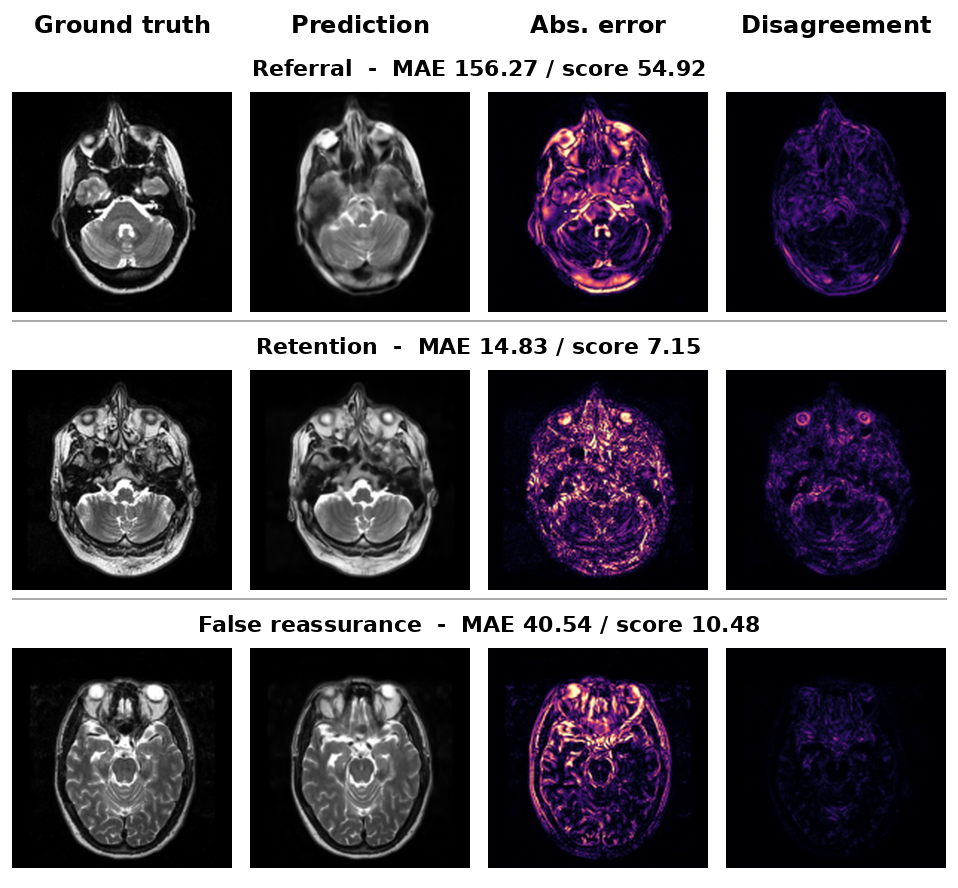
\includegraphics[width=0.82\textwidth]{qualitative_failures_relayout.png}
 \caption{Pre-defined qualitative categories from the frozen factor-four analysis: high-error flagged examination, low-error retained examination, and false reassurance. Panels visualize target, error, and disagreement under fixed display rules; examples illustrate behavior and are not used for selection.}
 \label{fig:qualitative-full}
\end{figure*}

Foreground definition can amplify these modes. A target-derived mask may exclude tissue the target has suppressed; a bank union may include noisy edges or background; an intersection can be too conservative. Input-derived masks avoid target circularity but depend on sparse-anchor coverage. The extended registry therefore retains target, bank-union, and observed-input supports. Ground-truth masks appear only in common-support offline sensitivity and model-fidelity labels. No deployment result uses them.

Intensity mismatch is handled as a scoring contract rather than silently optimized per cohort. Outputs are inverse-normalized to the source-volume representation before comparison. Independent percentile, robust location-scale, or min--max normalization can erase genuine amplitude disagreement, while raw output differences can react to model-wide brightness offsets. Gradient and local-energy variants reduce this sensitivity but did not survive nested transfer. We therefore retain raw target disagreement as the fixed cross-model baseline and state identical intensity representation as a necessary operating condition.

The most important negative findings are consequently part of the method definition: (i) committee consensus does not imply correctness; (ii) target specificity is weak after within-case calibration; (iii) high-dimensional adaptive selection is unstable in 22 examinations; (iv) physical consistency requires genuinely corresponding generated world planes and multiple factor outputs; and (v) neither MAE nor a reliability rank measures diagnostic harm. These boundaries constrain the intended use to retrospective prioritization and motivate future reader and downstream-task studies.

\clearpage
\section{Discussion and Conclusion}
Case ranking is stronger than voxel localization because foreground aggregation suppresses local noise while preserving between-examination severity. Physical consistency adds a distinct signal: it observes whether one reconstructor changes on the same world plane as sampling context changes. Its success does not rescue target attribution, and a high score may still flag correct but unusual detail.

The evidence has three levels. The original median disagreement, mask, and review metric were frozen before multiscale analysis. Physical matching and the 50/50 rank hybrid were specified before world-coordinate results were computed, so their nine-profile comparison is an evaluation of fixed formulas rather than per-profile selection. By contrast, the amended adaptive selector was introduced after diagnosing the analytical-only collapse; its complete outer results are retained but interpreted only as an exploratory sensitivity. This distinction prevents a negative first finalist from being silently replaced.

The physical score is attractive when a benchmark, model-comparison service, or retrospective audit already stores multiple factors. In a single-factor online system it requires two extra executions of the target reconstructor. Cross-model disagreement instead requires peer models, but analytical members are inexpensive and cached neural predictions amortize reconstruction cost. The hybrid has the highest online burden and should be used only when the observed ranking gain justifies this cost. None of the scores changes the reconstructed volume or autonomously rejects an examination; it only orders a review queue whose operating coverage is set by available human capacity.

Limitations are substantive. Shared blur, deletion, bias, or preprocessing failure can fool all members; correlated training data reduce committee diversity; masks can omit suppressed tissue; fastMRI-brain and NingXia are small; evidence is T2 brain MRI; and cross-scale scoring requires multiple reconstructions. MAE is not diagnostic harm, no reader or downstream study is available, and neither score is calibrated. We conclude that target-to-committee disagreement is a reproducible frozen review baseline and physical-plane consistency can strengthen multiscale examination ranking. Adaptive committee selection needs larger development cohorts; neither consensus nor consistency guarantees clinical correctness.

\clearpage
\bibliographystyle{IEEEbib}
\bibliography{references}
\end{document}
